\documentclass[tikz,border=10pt]{standalone}
\usepackage{pgfplots}
\pgfplotsset{compat=1.18}
\usepackage{amsmath,amssymb}
\usetikzlibrary{arrows.meta}

\begin{document}
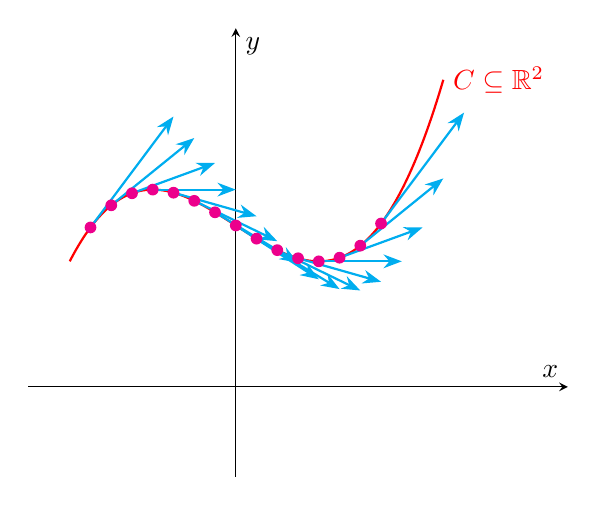
\begin{tikzpicture}
\begin{axis}[
axis lines=center,
xlabel={$x$}, ylabel={$y$},
xtick=\empty, ytick=\empty,
xmin=-2.5, xmax=4,
ymin=-5, ymax=20,
clip=false
]

% Plot the curve f(x) = x^3 - 3x + 9
\addplot[domain=-2:2.5, samples=200, thick, red] {x^3 - 3*x + 9};
\node[right, red] at (axis cs:2.5, {2.5^3 - 3*2.5 + 9}) {$C \subseteq \mathbb{R}^2$};

% Tangent vectors from point a
\pgfplotsextra{
	\foreach \a in {-1.75, -1.5, ..., 1.75} {
		\pgfmathsetmacro{\dx}{1}
		
		% Compute f(a) = a^3 - 3a + 9
		\pgfmathparse{\a*\a*\a - 3*\a + 9}
		\edef\ay{\pgfmathresult}
		
		% Compute f'(a) = 3a^2 - 3
		\pgfmathparse{3*\a*\a - 3}
		\edef\slope{\pgfmathresult}
		
		% Compute vector end point (a+dx, f(a)+slope*dx)
		\pgfmathparse{\a + \dx} \edef\endx{\pgfmathresult}
		\pgfmathparse{\ay + \slope*\dx} \edef\endy{\pgfmathresult}
		
		% Draw arrow
		\edef\cmd{
			\noexpand\draw[-{Stealth}, thick, cyan]
			(axis cs:\a,\ay) -- (axis cs:\endx,\endy); 
%			node[right] {$\langle 1, f'(\a)\rangle$};
		}
		\cmd
		
		% Mark point
		\edef\mark{
			\noexpand\node[circle, fill=magenta, inner sep=1.5pt]
			at (axis cs:\a,\ay) {};
		}
		\mark
		
		% Dashed guides
%		\edef\dashedX{
%			\noexpand\draw[dashed, magenta]
%			(axis cs:\a,\ay) -- (axis cs:\a,0);
%		}
%		\edef\dashedY{
%			\noexpand\draw[dashed, magenta]
%			(axis cs:\a,\ay) -- (axis cs:0,\ay);
%		}
%		\dashedX
%		\dashedY
	}
}
\end{axis}
\end{tikzpicture}
%\begin{tikzpicture}
%\begin{axis}[
%	axis lines=center,
%	xlabel=$x$,
%	ylabel=$y$,
%	xtick=\empty, ytick=\empty,
%	xmin=-2.5, xmax=4,
%	ymin=-5, ymax=20,
%	clip=false
%	]
%	
%	% Plot the curve f(x) = x^3 - 3x + 9
%	\addplot[domain=-2:2.5, samples=200, thick, red] {x^3 - 3*x + 9};
%	\node[right, red] at (axis cs:2.4, {2.4^3 - 3*2.4 + 9}) {$C \subseteq \mathbb{R}^2$};
%	
%	% Use pgfplotsextra to safely evaluate coordinates
%	\pgfplotsextra{
%		\foreach \a in {-2.5, -2, ..., 1.75} {
%			\pgfmathsetmacro{\dx}{.25}
%			
%			% evaluate function and derivative
%			\pgfmathparse{\a^3 - 3*\a + 9} \let\ay\pgfmathresult
%			\pgfmathparse{3*\a^2 - 3} \let\slope\pgfmathresult
%			
%			% compute end point of vector
%			\pgfmathparse{\a + \dx} \let\endx\pgfmathresult
%			\pgfmathparse{\ay + \slope * \dx} \let\endy\pgfmathresult
%			
%			% draw vector from (a, f(a)) to (a+dx, f(a)+f'(a) dx)
%			\edef\drawcmd{
%				\noexpand\draw[->, thick, cyan]
%				(axis cs:\a,\ay) -- (axis cs:\endx,\endy);
%			}
%			\drawcmd
%%			% f(a)
%%			\pgfmathparse{\a^3 - 3*\a + 9}
%%			\let\ay\pgfmathresult
%%			
%%			% f'(a)
%%			\pgfmathparse{3*\a^2 - 3}
%%			\let\slope\pgfmathresult
%%			
%%			\pgfmathsetmacro{\dx}{1}
%%			\pgfmathparse{\a + \dx} \let\endx\pgfmathresult
%%			\pgfmathparse{\ay + \slope*\dx} \let\endy\pgfmathresult
%%			
%%			% draw vector
%%			\edef\drawcmd{
%%				\noexpand\draw[-{Stealth}, thick, cyan]
%%				(axis cs:\a,\ay) -- (axis cs:\endx,\endy);
%%			}
%%			\drawcmd
%%			
%%			% draw point
%%			\edef\markcmd{
%%				\noexpand\node[circle, fill=magenta, inner sep=1.5pt] at (axis cs:\a,\ay) {};
%%			}
%%			\markcmd
%%			
%%			% projections
%%			\edef\dashedX{
%%				\noexpand\draw[dashed, magenta] (axis cs:\a,\ay) -- (axis cs:\a,0);
%%			}
%%			\edef\dashedY{
%%				\noexpand\draw[dashed, magenta] (axis cs:\a,\ay) -- (axis cs:0,\ay);
%%			}
%%			\dashedX
%%			\dashedY
%		}
%	}
%\end{axis}
%\end{tikzpicture}
\end{document}
